\chapter{Physics Objects}

In this chapter the algorithms used to reconstruct analysis objects and
quantaties from individual measurements from different parts of the CMS detector
are described.

\FigureRef{reco:crosssec} shows a cross section of CMS super imposed with the
typical paths of several different particles.

\begin{figure}[htb]
  \centering
  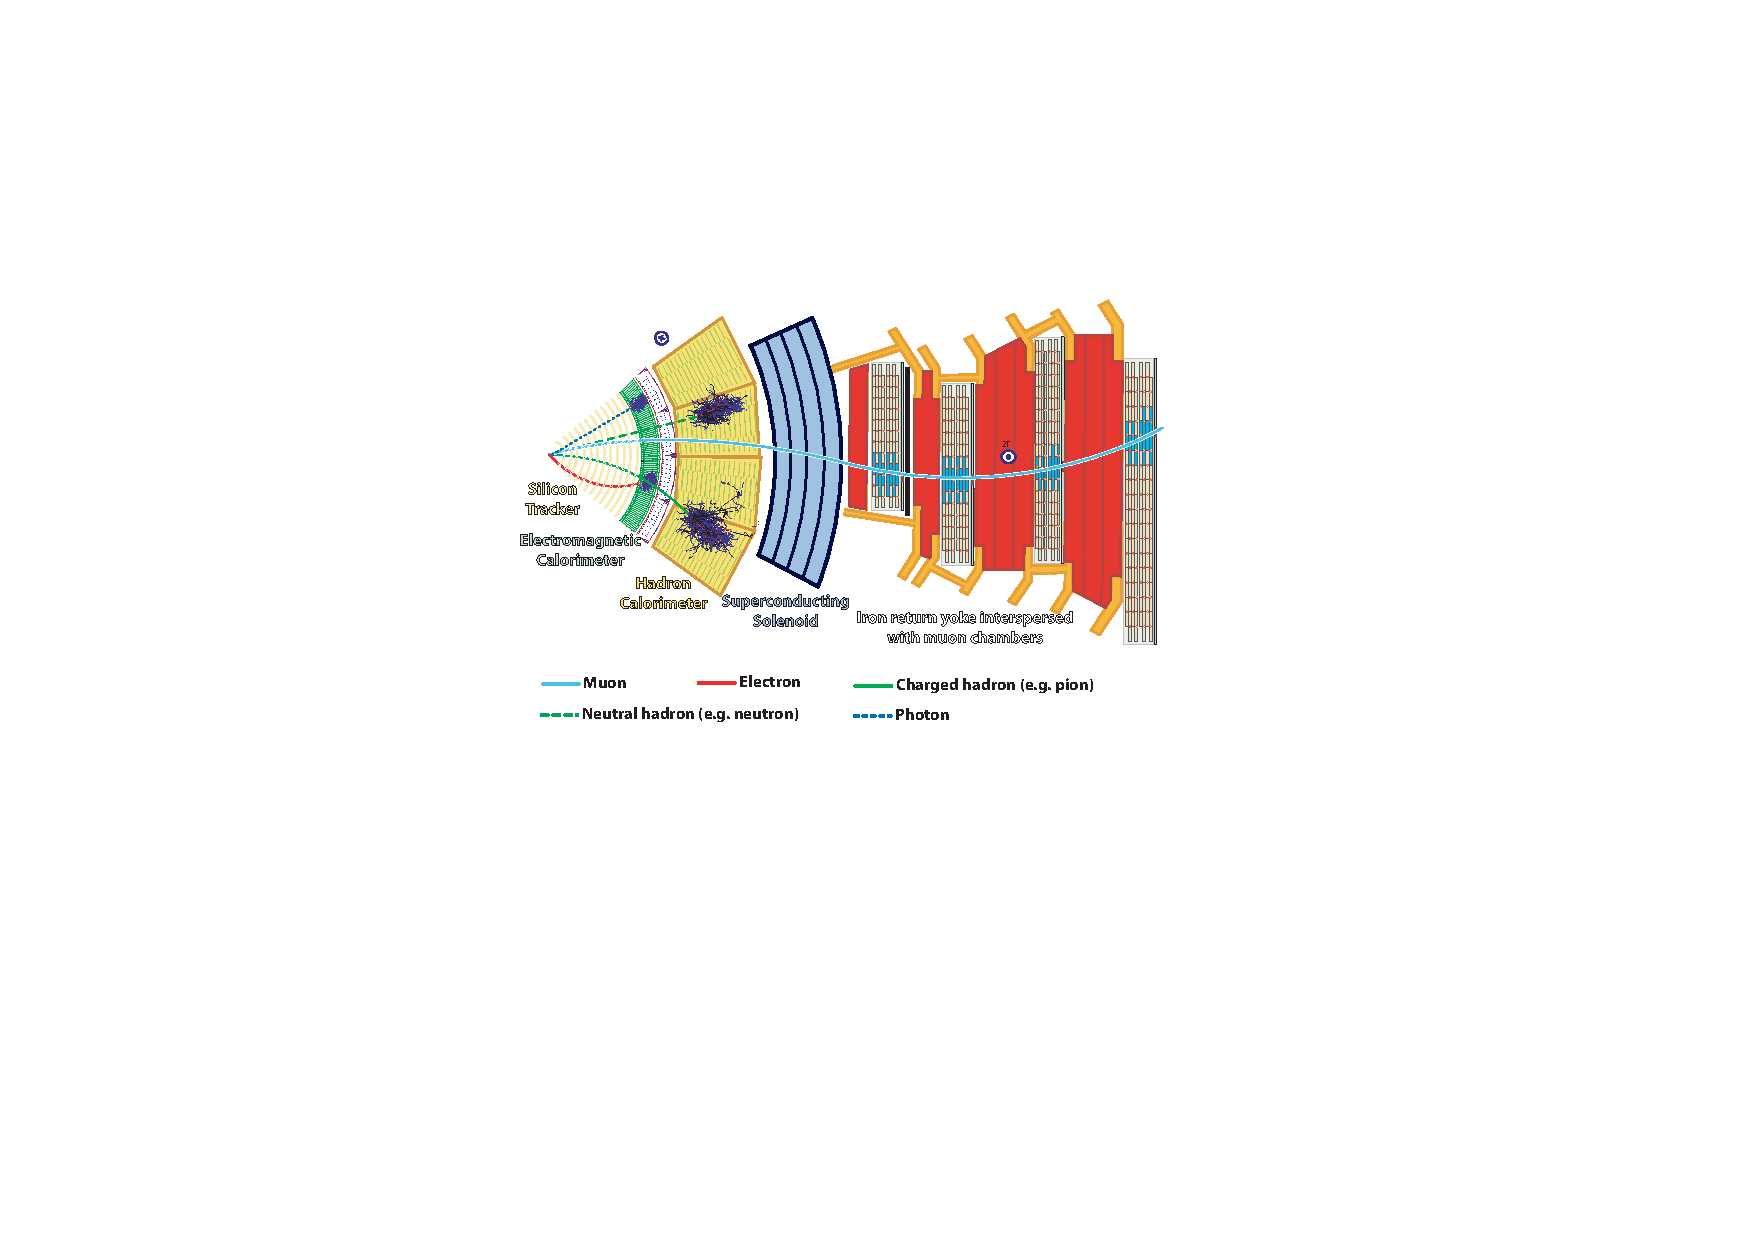
\includegraphics[trim=8cm 8cm 8cm 5cm, width=\textwidth]{slice}
  \caption{The path of different particles through a cross section of the CMS detector.}
  \label{reco:crosssec}
\end{figure}

\section{Electrons}

Electrons are important physics objects in CMS. They are easy to identify and
their energy can be measured with a good resolution. This section will describe
the electron reconstruction algorithms used to produce electron candidates, and
the identification variables used to discriminate between real electron
candidates and their background.

\subsection{Reconstruction}
Electrons are reconstructed in CMS using information from the pixel detector,
silicon strip tracker and the ECAL.
The first step of the reconstruction is to collect together energy deposits in
the ECAL. Next, the path of the electron though the tracker is reconstructed and
the matched to the energy deposits in the ECAL.

\subsubsection{Electron Clustering}
As electrons traverse the CMS tracker, the strong magnetic field causes the path
of the electrons to be curved in the azimuthal, $\phi$, direction. The electrons
radiate bremsstrahlung photons, so that when the electron energy reaches the
ECAL it is spread over a narrow strip in the phi direction.
\FigureRef{reco:brem} shows the fraction of energy radiated by bremsstrahlung for
electrons of energy $10$, $30$ and \unit{$50$}{\GeV}.

\begin{figure}[htb]
  \centering
  %
\includegraphics[width=0.5\textwidth]{placeholder}
  \missingfigure{Fraction of energy radiated by bremsstrahlung from Electron
reconstruction in CMS}
  \caption{Fraction of electron energy, $E^{e}$, radiated away as bremsstrahlung
photons, $\sum E_{brem}^{\gamma}$ for electrons of energy }%$10$, $30$ and \unit{$50$}{\GeV}. From \cite{}.}
  \label{reco:brem}
\end{figure}

To measure the electron energy, including the bremsstrahlung photons, the
seperated deposits of energy need to be collected together, using super-clustering
algorithms. 

In the barrel a ``hybrid'' algorithm is used. The hybrid algorithm proceeds by
identifying several hot crystals, with energies above a certain threshold, that
will act as seeds. The algorithm then forms $1\times3$ or $1\times5$ crystal
``dominos'', centered on the seed crystal, depending on the energy within the
domino. The dominos are then collected together in the $\phi$ direction, up to
an extension of \unit{0.3}{\rad}, to form clusters of clusters. This is
demonstrated in \FigureRef{fig:hybrid}.

\begin{figure}[htb]
  \centering
  %
\includegraphics[width=0.5\textwidth]{placeholder}
  \missingfigure{hybrid clustering algorithm}
  \caption{Demonstration of the clustering of dominos in the hybrid algorithm.}
  \label{reco:hybrid}
\end{figure}

A ``multi5x5'' algorithm is used in the ECAL endcaps. Energy is collected in
$5\times5$ matrices, which are then collected together if their position lies on
a narrow $\phi$ road to form superclusters.

\subsubsection{Electron Seeding}
The superclusters are then used to select seeds for the track reconstruction.
Starting with a supercluster that passes a \pt and a hadronic veto, the
trajectory of the electron is propogated back through the magnetic field and
matched to the trajectory seeds, pairs or triplets of hits in the inner tracker.
If the trajectory seeds fall within a window of the supercluster path under
either charge hypothesis, they are selected and used to seed the track
reconstruction.
The ECAL driven seeding is comlemented by a tracker driven seeding algorithm.
This starts with high purity tracks and extrapolating them outwards to the ECAL.
This is effective for lower \pt electrons.

Seeds from both of the algorithms are collected and merged in to a single
collection, which is then used to seed the electron track reconstruction.

\subsubsection{Electron Track Reconstruction}
The track reconstruction is based on a combinatorial Kalman filter,\todo{find a
citation for this} with the electron energy losses described using Bethe Heitler
modelling.

The track reconstruction starts with a seed, from which a tree of possible track
candidates is built from. 

%track reconstruction paper
Throughout the track reconstruction, tracks candidates are described by a state
vector containing information on the momentum, direction and position of the
track.

The Kalman filter is a
two step process. In the propogation step, track states are extrapolated to
the next layer of the detector, while taking in to account for energy losses due
to bremsstrahlung and coulomb scattering. 
In the update step, the extrapolated track state is 
combined with what is observed in that layer and the track is updated. 

The collected hits are passed to the GSF for a final fitting and estimation of
the track parameters. The GSF algorithm is similar to the Kalman filter but
energy losses are now described by a weighted sum of Gaussian distributions.
% corrections

\subsection{Backgrounds to Prompt Electrons}
In addition to prompt electrons, the electron candidates from the reconstruction
algorithms will contain background signatures, either fake electrons or unwanted
real electrons produced via some background process.

There are two main processes that may produce signatures in the detector that
may be mistakenly identified as an electron and an additional
two processes that may produce real electrons.
\cite{Nikos}

\subsubsection{Charged hadrons that shower early in the ECAL}
A charged pion will leave a track, that will appear similar to an non-radiating
electron track. If the pion were to produce a hadronic shower early in the ECAL
the energy deposits in the ECAL would be indistiguishable from an
electromagnetic shower.

\subsubsection{\HepProcess{\Ppipm \Ppizero} overlap}
A charged pion within a jet will produce a charged track where as a neutral pion
will quickly decay to a pair of photons. If the electromagnetic clusters from
the \Ppizero are matched to the track from the charged hadron, the electron
reconstruction algorithm may form an electron candidate.

\subsubsection{Electrons from hadronic decays}
Heavy flavour quarks may decay semileptonically to produce real electrons. These
electrons will tend to be less well isolated than prompt electrons from \PW
decays.

\subsubsection{Electrons from conversions}
As stated previously, a neutral pion will produce a pair of photons. As the
photons traverse the tracker material they may convert to produce a pair of real
electrons. These electrons will tend to have missing hits close to the
interaction point and a partner track nearby with opposite charge.

\subsection{Electron Identification}
Electron identifiaction is based on a limited number of variables.

\subsubsection{Shape variable}

$\sigma_{\eta\eta}$ is the width of the electron shower in the $\eta$
direction\todo{this might be wrong}
\begin{equation}
\sigma_{\eta\eta} = 
\sum_{\text{crystals}} \left(\eta_{i} - \eta{s}\right)^{2}
\frac{E_{i}}{E_{\text{seed cluster}}}.
\end{equation}
This variable descriminates between prompt electrons and jets, as a hadronic
shower from a jet or a pair of photons from a \Ppizero will tend to produce a
wider electromagnetic shower than an electron.

\subsubsection{Hadronic energy}
Ratio of the energy deposited in the HCAL tower behind the electromagnetic seed
cluster to the energy of that seed cluster. This variable offers some
discrimination against early showering hadrons as some of the energy will tend
to leak in to the HCAL.

\subsubsection{Angular separation of track and super cluster}
$\Delta\phi$ and $\Delta\eta$ represent the angular separation between the
trajectory of the reconstucted GSF track, extrapolated to the ECAL, and the ECAL supercluster in the $\phi$
and $\eta$ direction respectivly.
\begin{align}
|\Delta\eta| &\equiv |\eta_{\text{SC}} - \eta_{track}|\\
|\Delta\phi| &\equiv |\phi_{\text{SC}} - \phi_{track}|
\end{align}
These variables are discriminating against accidental matching to the track and
supercluster.

\subsubsection{Isolation quantaties}
For the calorimeter quantities the isolation is defined as the some of energy in
a cone of $\Delta R = 0.3 $ centered on the super cluster, where the energy
deposits associated with the electron have been removed, divided by the
candidate electron \Pt.

The track isolation is defined as the sum of the \Pt of Kalman filter tracks in
a cone of $\Delta R = 0.3 $ centered on the candidate electron, divided by the
candidate electron \Pt.

Isolation offers very good discrimination between electrons and hadrons, as
hadrons that are mistakenly identified as an electron will tend to be
accompanied by other particles, where as prompt electrson will usually be well
isolated.

\subsubsection{Conversion rejection}
Three further variables are included to reject electrons that are produced from
photon conversions, missing hits, $\Delta\cot\theta$ and dist. 

The missing hits is simply the number of layers in the inner
tracker where an expected hit from the track reconstruction is not detected by
the detector.

Two other variables are based on conversion partner tracks.
Coversion partner tracks are track candidates that are with in a cone of $\Delta
R < 0.3$ around the electron candidate track, and have an opposite charge. 
$\Delta\cot\theta$ is defined as,
\begin{equation}
\Delta \cot \theta \equiv \cot(\theta_{\text{KF}}) - \cot(\theta_{\text{GSF}}),
\end{equation}
where $\theta_{KF}$ and $\theta_{GSF}$ are the polar angle of the conversion
partner track and the GSF track of the electron respectivly.
The variable, dist, is the distance between the two tracks where they are
parralel as described in \FigureRef{fig:dist}.

\begin{figure}[htb]
  \centering
  \missingfigure{Explanation of dist}
  %
\includegraphics[width=0.5\textwidth]{placeholder}
  \caption{Dist is the distance between}
  \label{fig:dist}
\end{figure}

\subsubsection{Electron identification working points}

Several sets of cuts have been produced for CMS analyses with different
efficiencies in mind. The cut values are sumarised in \TableRef{tab:electronwp}.
\todo{table of electron working points}

\subsection{Charge Identification}
The charge of an electron can be identified by studying how the electron trajectory
is bent in the magnetic field as the electron passes through the tracker. This
can be made difficult by conversion of bremsstrahlung photons when they are
radiated early.\todo{explain this} 

Within CMS, three methods of charge identifaction have been developed based on
the GSF track charge, the general track charge and the supercluster charge. The
GSF track charge is simply the sign of the curvature of the GSF fit of the
electron track. The general track charge is found by matching the GSF track with
general Kalman filter track by asking for shared hits in the pixel tracker. 
The super cluster charge is obtained by finding the sign of the phi difference
between the supercluster position and the first hit of the electron track.

At the \PZ peak, a charge mis-identification rate of \unit{3}{\%}\todo{cite this} is expected,
when using the electron trajectory from the GSF fit.  A sample with improved
charge identifaction can be obtained by using a majority method, that combines
the three measurements and assigns the sign from the 2 estimates out of three
that are in agreemenet, or by requiring that all three methods for assigning
charge are in agreement and discarding the event otherwise.
\todo{plots here?}

\section{Missing Energy} 
Neutrinos are weakly interacting neutral particles and escape the
detector with out being directly detected by any of the detector components. 
Instead they can be indirectly detected by measuring the total momentum of the
reconstructed particles in an event.
An imbalance in the total momentum of the event can be assigned to undetected
particles, this is the missing energy in the event.

Unfortunatly the initial longditudianl momentum of the event is not known in a
hadron collider, so instead the inbalance in only the transverse plane is
considered. This is the missing transverse energy, \ETm, and is defined as
the negative vector sum of all final state particles in an event,
\begin{equation}
\ETm = -\sum_i^{\text{particles}} \vec{p}_{T}^{i}.
\end{equation}

There are several ways of measuring the missing transverse energy.

Calo \ETm is measured by creating pseudo-particles from the energies and
direction of deposits in the calorimeter towers. The muons are included by
adding their \Pt to the calculation and removing their energy deposit in the
calorimeter. The calo \ETm is then the sum of the transverse energy of the
pseudo particles.

Track \ETm is extends calo \ETm to include the track \Pt and remove the energy
deposit for each track in the event.

Particle Flow \ETm (PF \ETm) is the sum of the transverse energies of all the
reconstructed particle flow particles.

\subsection{Particle Flow at CMS}

The particle-flow event reconstruction attempts to reconstruct and identify all
stable particles in an event by combining information from all CMS
sub-detectors. The particle reconstruction and identification starts with
collecting information from each subdetector to form elements such as tracks
and energy clusters in the calorimeters. These basic 'elements' are then
combined to form blocks which are then interpreted in terms of particles by the
particle flow algorithm. A list of individual particles is then returned from
the algorithm which can be used to study the event in greater detail by,
amongst other things, building jets, tagging b quarks and calculating missing
transverse energy.\cite{PF}

The first step of the particle-flow reconstruction algorithm is to collect the
fundamental elements. The elements consist of charged particles tracks from the
tracker, clusters of energy deposition in the calorimeters and muon tracks.
These elements need to be identified with a high efficiency and low fake rate
since the particle reconstruction depends on these basic elements and
misidentified elements could lead to missing or double counted
particles.\cite{PF}

As a particle traverses the detector it may interact with many CMS subdetectors
creating several particle-flow elements. A link algorithm is used to connect
the elements together to form blocks that typically contain 1, 2 or 3 elements.
The algorithm returns a distance between the elements as a measure of the
quality of the link. The final step of the particle flow algorithm is to
reconstruct and identify particles from each block of linked elements.\cite{PF}

Once the event has been fully reconstructed with the particle flow technique
the missing transverse energy (\ETm) in the event can be easily computed by
summing up the transverse momentum of all the reconstructed particles.\cite{PF}

